% !Mode:: "TeX:UTF-8"
\chapter{Исследование методов построения системных тестов}

\section{Системное тестирование микропроцессоров}

Прежде, чем описывать методы построения системных тестов (т.е. тестов, которые используются для системного тестирования), следует дать понятие о самом системном тестировании более чётко.
\begin{figure}[h] \center
  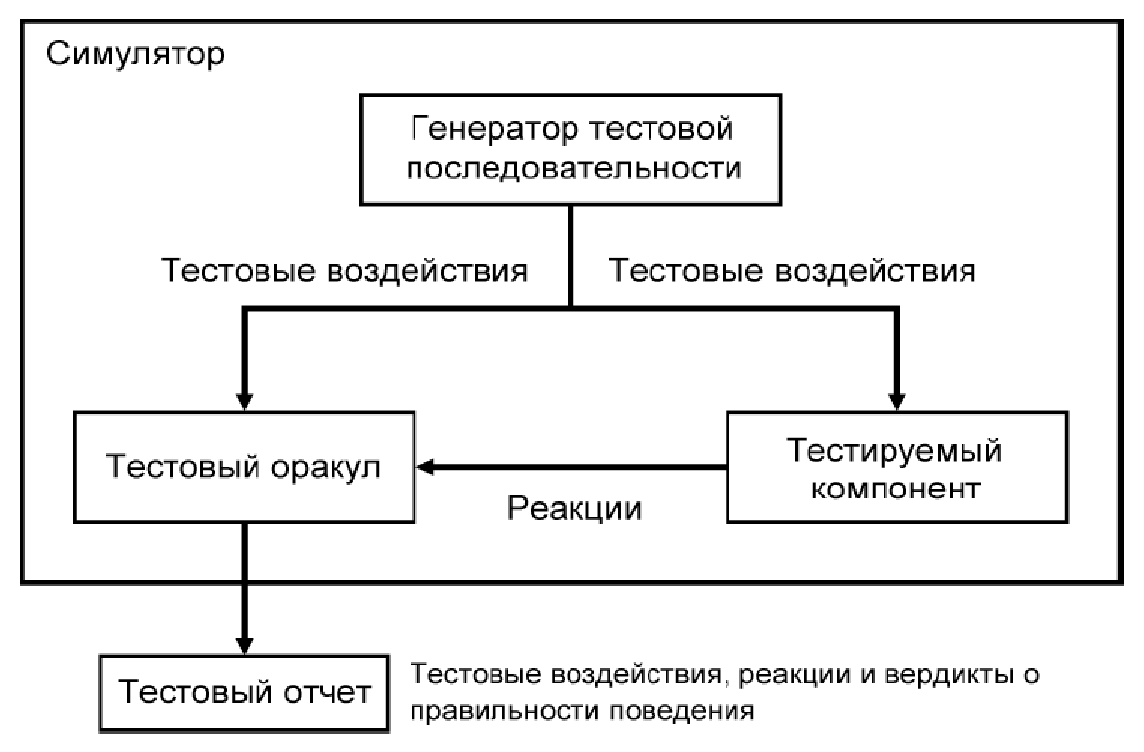
\includegraphics[width=0.7\textwidth]{1.review/test-system}\\
  \caption{Архитектура тестовой системы}\label{fig:test_system}
\end{figure}

На рисунке~\ref{fig:test_system} приведена архитектура тестовой системы, общеупотребительная как для аппаратного, так и для программного обеспечения~\cite{IvanPreprint} (везде, где говорится об аппаратном обеспечении, подразумеваются их программные модели на языках Verilog/VHDL). Генератор тестовой последовательности строит \emph{тестовые воздействия} (в случае системного тестирования это программы на машинном языке) и передает их на тестируемый компонент (каждая сгенерированная программа запускается на программной модели микропроцессора). В результате тестируемый компонент выдает \emph{реакцию} (в случае системного тестирования это значения регистров в разное время, состояние блоков кэш-памяти, таблицы страниц, происходившие исключительные ситуации и т.п.). Реакция и те же тестовые воздействия передаются \emph{тестовому оракулу}, задачей которого является оценка соответствия полученной реакции тестовому воздействию (что из себя представляет тестовый оракул в случае системного тестирования будет сказано чуть позже). В результате своей работы тестовый оракул составляет \emph{тестовый отчет}, в котором отражено какие подавались тестовые воздействия (точнее, из каких классов подавались тестовые воздействия), какие получены реакции и каковы были вердикты оценки их соответствия.

Тестовый оракул (в случае системного тестирования) может быть построен следующими способами:
\begin{itemize}
  \item \emph{ко-симуляция}~\cite{HoPhD}: разрабатывается программная модель тестируемого микропроцессора, более простая, нежели тестируемая (эмулятор микропроцессора, интерпретатор системы команд); обычно такие модели разрабатываются на языках высокого уровня (например, Си или Си++) людьми, не занятыми в разработке тестируемой программной модели (для исключения возможности одинаковых ошибок в обеих моделях); тестовый оракул подает переданные ему тестовые воздействия на эту <<эталонную>> модель, получает ее реакции и сравнивает их с реакциями тестируемой модели;

  \item \emph{самопроверяющие тесты}~\cite{HoPhD}: реакция тестируемой модели уже содержит в себе вердикт, поэтому тестовый оракул напрямую использует его для составления тестового отчета; например, это тесты, в которых (как следует из названия) содержатся необходимые проверки состояния в результате тестового воздействия (например, проверяется, что заданные регистры получили нужные значения);

  \item \emph{на основе формальных спецификаций}~\cite{KamkinThesis}: тестовый оракул использует технику пред- и пост-условий для определения соответствия переданных ему тестовых воздействий и реакций.
\end{itemize}

Тестовый отчет отражает, насколько полно было произведено тестирование. Оценка полноты тестирования производится на основе метрик покрытия. Метрики покрытия, в свою очередь, формулируются на основе критерия покрытия. Критерий покрытия определяет, что будет пониматься под \emph{тестовой ситуацией}. Например, критерием покрытия может быть покрытие всех строк программной модели микропроцессора. В результате тестирования может быть сделан вывод, что достигнуто покрытие 90\% ситуаций согласно этому критерию. Иными словами, при тестировании было задействовано 90\% строк программной модели микропроцессора. Каждая строка задавала свою тестовую ситуацию.

Методы автоматической генерации тестов (тестовых воздействий) делят на псевдослучайные/комбинаторные (pseudo-random) и целенаправленные (что не отменяет возможности использования уже готовых тестов)~\cite{HoPhD}. В случае псевдослучайной генерации инструкции, их порядок и аргументы выбираются случайным образом или перебираются некоторым комбинаторным способом. В методах целенаправленной генерации все тестовые ситуации неким \emph{систематическим} образом перебираются и для каждой ситуации \emph{нацеленным образом} строится тестовое воздействие (т.е. в этом тестовом воздействии будет обязательно воспроизведена эта ситуация).

Эффективность тестирования будет ниже, если многие построенные тестовые воздействия будут соответствовать одной ситуации. В этом случае для получения полного покрытия пространства тестовых ситуаций придется использовать больше тестов. Эта проблема особенно актуальна в случае псевдослучайной генерации тестов, поскольку в ней не гарантируется покрытие заданных ситуаций.

По соображениям эффективности целенаправленные методы генерации тестов представляют б\textit{o}льшую актуальность и данная работа посвящена исследованию этого класса методов автоматического построения тестов. Далее под \emph{нацеленными тестами} будут пониматься тесты, построенные нацеленным образом. Все остальные тесты будут называться \emph{ненацеленными}. Если речь идет только о тестах для ситуаций в работе не всего микропроцессора, а его части (той же подсистемы управления памяти), то будем говорить о тестах, \emph{нацеленных на эту часть}, например, о тестах, нацеленных на подсистему управления памяти.

%Поскольку количество различных аспектов в работе микропроцессора (инструкций, их способов выполнения, особых режимов) измеряется десятками и сотнями, а кроме того из-за наличия конвейера в современных микропроцессорах в качестве ситуаций надо рассматривать не только аспекты, но и их комбинации. Поэтому количество различных ситуаций для всего микропроцессора это десятки и сотни тысяч.

%тестовые ситуации на основе ситуаций на конвейере и модели ошибок дают идею о том, что ситуации можно выражать в виде шаблонов программ....

%Целенаправленная генерация начинается с задания некоторого шаблона тестовой программы, который определяет набор инструкций, их последовательность и аргументы. В рамках целенаправленной генерации порядок инструкций и их аргументы должны быть подобраны таким образом, чтобы каждый новый тест покрывал новые, еще не покрытые тестовые ситуации. Целенаправленную генерацию можно реализовать как выполнение массовой генерации комбинаторных тестов с последующей фильтрацией, с тем чтобы оставлять только те тесты, которые дают дополнительное покрытие. Однако уже для достаточно коротких шаблонов (длиной 3-4 инструкции) перебор становится слишком большим.

%Целенаправленная генерация тестов дает по тесту на каждую ситуацию. Набор тестов, которые покрывают все ситуации, называют нацеленными тестами (нацеленными на эти ситуации). Набор ситуаций конечен, следовательно и набор нацеленных тестов конечен. Вопрос

%%(это и есть основная тема исследования)
%, как систематическим образом строить тестовые программы, чтобы в совокупности они воспроизвели все заданные <<интересные>> ситуации.


%Сложность микропроцессора определяет количество системных тестов. Если выделить различные аспекты функционирования микропроцессора (конвейер, буферы подсистемы управления памяти), то особое функционирование возникает при различных комбинациях этих аспектов. Это означает, что количество тестов должно быть не меньше произведения количества разных аспектов. Количество инструкций измеряется сотнями, а цепочек инструкций, соответственно, порядками сотен, плюс если учесть возможные аспекты в конвейере, в кэш-памяти, количество тестов получается очень большим. Для избежания проблемы такого <<взрывного>> характера количества тестов, их объединяют в классы эквивалентности --- \emph{тестовые ситуации}.

%При этом есть проблема покрытия всех потенциально интересных тестовых ситуаций. Нет никаких прямых способов создать многие из таких ситуаций нет. Например, интересно, как происходит доступ в память, когда соответствующий адрес имеется в кэш-памяти или не имеется. Или еще более тонкий анализ --- адрес имеется/или не имеется в кэш-памяти второго уровня. Среди инструкций процессора нет таких, которые были бы предназначены специально для создания таких ситуаций. Эти ситуации создаются \emph{динамически} в ходе выполнения программ.

%Микропроцессор рассматривается как черный (или серый) ящик. Входными тестовыми данными является некоторая программа, которая загружается в память. Результатом прогона теста является либо финальное состояние памяти (возможно, включая состояние регистров) или (в случае <<серого ящика>>) трасса изменения значений ячеек памяти или регистров.
%В этой общей схеме тестирования пока не упомянуты:
%\begin{itemize}
%	\item	генератор тестов (или набор уже готовых тестов);
%	\item	подсистема проверки корректности полученного результата --- тестового оракула, или арбитра;
%	\item	перечень <<интересных>> ситуаций, которые надо воспроизвести в ходе выполнения тестов;
%	\item	некая система мониторинга, которая фиксирует прохождение <<интересных>> ситуаций --- оценивает полноту покрытия.
%\end{itemize}
%
%Тестовый оракул, или арбитр, строится по схеме с использованием <<эталонной>> модели (simulation-based verification)~\cite{SimulationBased}. Каждая тестовая программа выполняется на двух моделях --- на тестируемой (design) и на <<эталонной>>. Потом состояния памяти или трассы изменения состояния памяти для тестируемой и эталонной моделей сравниваются. Если оракул признает, что трассы не эквивалентны, это свидетельствует о наличии ошибки в тестируемой системе (или эталонной, но это происходит реже). Как правило, эталонная модель пишется на одном из языков программирования (например, Си или Си++) и не загромождается деталями.  На этом основании считается, что такая модель существенно проще тестируемой, в ней с меньшей вероятностью встречаются ошибки, именно поэтому к ней можно относиться как к <<эталонной>>.
%
%% критика этого подхода: он не позволяет проверить модули, работающие за счет внешних воздействий - For example, fast interrupt request (FIQ), interrupt request (IRQ), data abort exception (Dabort) and prefetch abort exception (Pabort) of ARM7. Это пишут в статье "Automatic Verification of External Interrupt Behaviors for Microprocessor Design", авторы Fu-Ching Yang, Wen-Kai Huang, Ing-Jer Huang.
%
%
%Методы автоматической генерации тестов делят на псевдослучайные/комбинаторные (pseudo-random) и целенаправленные (что не отменяет возможности использования уже готовых тестов)~\cite{HoPhD}. В случае псевдослучайной генерации инструкции, их порядок и аргументы выбираются случайным образом или перебираются некоторым комбинаторным способом. Целенаправленная генерация начинается с задания некоторого шаблона тестовой программы, который определяет набор инструкций, их последовательность и аргументы. В рамках целенаправленной генерации порядок инструкций и их аргументы должны быть подобраны таким образом, чтобы каждый новый тест покрывал новые, еще не покрытые тестовые ситуации. Целенаправленную генерацию можно реализовать как выполнение массовой генерации комбинаторных тестов с последующей фильтрацией, с тем чтобы оставлять только те тесты, которые дают дополнительное покрытие. Однако уже для достаточно коротких шаблонов (длиной 3-4 инструкции) перебор становится слишком большим.
%
%Целенаправленная генерация тестов дает по тесту на каждую ситуацию. Набор тестов, которые покрывают все ситуации, называют нацеленными тестами (нацеленными на эти ситуации). Набор ситуаций конечен, следовательно и набор нацеленных тестов конечен. Вопрос
%%(это и есть основная тема исследования)
%, как систематическим образом строить тестовые программы, чтобы в совокупности они воспроизвели все заданные <<интересные>> ситуации.
%
%
%Перечень (конечный) <<интересных>> ситуаций и мониторинг. В совокупности две эти возможности задают метрику и механизм оценки полноты тестирования. Мониторинг организовать относительно легко, поскольку мы работаем не с реальным процессором, а с его моделями. Как построить перечень «интересных» ситуаций» --- вопрос открытый --- это одно из направлений моей работы.


\section{Тестирование подсистем управления памяти}\label{section:cache}

Подсистема управления (механизмами) памяти (MMU, Memory Management Unit) ---
логически связанный набор модулей микропроцессора, который выполняет
функции обращения к памяти~\cite{MMU}. Практически ни один
микропроцессор не обходится без MMU.

Основными функциями MMU являются:
\begin{enumerate}
  \item \emph{трансляция адресов}: преобразование логических адресов в физические;
  \item \emph{организация виртуальной памяти};
  \item \emph{организация защиты} адресного пространства процесса от других процессов;
  \item \emph{организация кэширования данных оперативной памяти} (иногда эту функцию включают в MMU~\cite{vorobyev},~иногда --- нет~\cite{thompson}).
\end{enumerate}

Согласно этим функциям MMU в число модулей, которыми она управляет, включаются:
\begin{itemize}
  \item кэш-память (кэш-память данных и кэш-память инструкций)  первого и более высоких уровней;
  \item TLB (Translation Lookaside Buffer) -- буфер, задающий
  соответствие некоторых страниц виртуальной памяти кадрам
  физической памяти;
  \item таблица страниц -- различным образом организованное полное соответствие всех страниц виртуальной памяти кадрам физической памяти;
  \item сегментные регистры (содержат логические адреса начала сегментов);
  \item различные другие буферы.
\end{itemize}

%Организация кэширования в MMU отличается от организации кэширования
%программных систем (баз данных, операционных систем) тем, что в микропроцессорах
%применяется довольно ограниченный набор стратегий вытеснения. Наиболее часто применяются
%стратегии вытеснения \LRU, \FIFO и \PseudoLRU. Это связано с особыми требованиями
%к эффективности реализации алгоритмов вытеснения в микропроцессорах (вся реализация
%алгоритма вытеснения должна располагаться на кристалле и не давать большой проигрыш по времени).

Кэш-память хранит набор блоков данных (кэш-строк). Каждому блоку данных соответствует адрес (физический или виртуальный), все такие адреса разные. Зачастую блоки данных, кроме адреса, снабжаются другой служебной информацией (например, флаги).

Кэш-память призвана ускорить доступ к данным, хранящимся в оперативной памяти. Если во время доступа данные по нужному адресу нашлись в кэш-памяти, то обращение в оперативную память не производится. Чтобы нужные данные оказались в кэш-памяти, они должны быть туда помещены. Чтобы при этом кэш-память не увеличивалась в размерах (что чревато понижением ее эффективности), начиная с некоторого ее размера, перед добавлением блока новых данных из кэш-памяти удаляется один из находящихся в ней блоков данных (этот процесс называется \emph{вытеснением}), добавление происходит на место вытесненного блока данных.

Функциональность кэш-памяти определяется в виде набора \emph{стратегий} (policy):
\begin{itemize}
	\item \emph{стратегия кэширования (write policy)} (встречается также прямая транскрипция англоязычного термина, как <<политика записи>>)
		\begin{itemize}
		\item при некэшируемом обращении (uncached) кэш-память не используется;
		\item при кэшируемом обращении со сквозной записью (write-through) инструкция сохранения данных в памяти изменяет соответствующий блок данных как в кэш-памяти, так и в оперативной памяти;
		\item при кэшируемом обращении с обратной записью (write-back) инструкция сохранения данных в памяти изменяет соответствующий блок данных только в кэш-памяти, а изменение данных в оперативной памяти откладывается;
		\end{itemize}
	\item \emph{стратегия вытеснения (replacement policy)} (встречается также прямая транскрипция англоязычного термина, как <<политика замещения>>) --- правило определения вытесняемого блока данных; примеры --- согласно \LRU (Least Recently Used) вытесняется блок данных, к которому дольше остальных не было обращений, согласно \FIFO (First-In First-Out) вытесняется блок данных, добавленный в кэш-память позже остальных;
	\item \emph{стратегия чтения (read architecture)}~\cite{IntelCache}:
		\begin{itemize}
			\item при сквозном доступе (look-through) запрос сначала производится только в кэш-память и при неуспехе производится еще один запрос, на этот раз в оперативную память или другие уровни кэш-памяти;
			\item при побочном доступе (look-aside) одновременно отправляются запросы во все уровни кэш-памяти и в оперативную память;
		\end{itemize}
	\item \emph{стратегия помещения данных}~\cite{Kasperski_EffectiveMemory} определяет, надо ли (и когда) при промахе помещать данные из оперативной памяти в кэш-память; микропроцессоры Intel Pentium и AMD всегда помещают такие данные в кэш-память;
	\item \emph{включающая/исключающая организация}:
		\begin{itemize}
		\item включающая организация (inclusive) предполагает при промахе в одном уровне кэш-памяти добавлять нужные данные и во все более быстрые уровни кэш-памяти; этой архитектуре следуют микропроцессоры AMD K6, Pentium II, Pentium III~\cite{Kasperski_EffectiveMemory};
		\item исключающая организация (exclusive) обеспечивает, что один и тот же блок данных не хранится в нескольких уровнях кэш-памяти одновременно; ей следует микропроцессор AMD Athlon~\cite{Kasperski_EffectiveMemory}.
		\end{itemize}
\end{itemize}

Блоки данных кэш-памяти организованы в \emph{секции} и \emph{наборы} (см.рис.~\ref{fig:cache_model}). Один набор образуют блоки, которые определяют вытеснение друг друга. Т.е. блоки, не входящие в набор вытесняющих данных, не могут быть вытеснены. Какой набор будет задействован для данного адреса, определяется только на основе этого адреса. Номер соответствующего набора является функцией адреса. В каждом наборе одинаковое количество блоков данных. Каждый такой блок относится к одной из секций. Деление блоков по секциям сделано лишь для ускорения поиска данных. А именно, поиск данных в блоках набора идет одновременно во всех секциях.

\begin{figure}[h] \center
  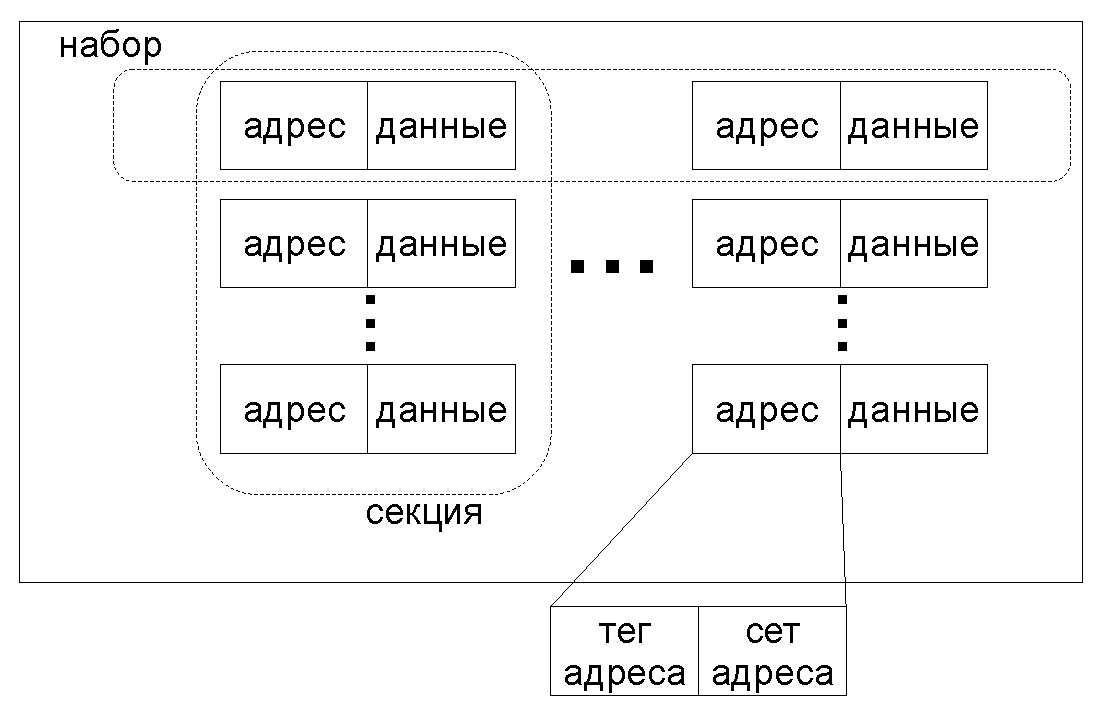
\includegraphics[width=0.7\textwidth]{1.review/cache}\\
  \caption{Схема кэш-памяти и адреса данных}\label{fig:cache_model}
\end{figure}

По структуре выделяют следующие три типа кэш-памяти:
\begin{itemize}
   \item \emph{полностью ассоциативная} кэш-память;
   \item кэш-память \emph{прямого доступа};
   \item \emph{наборно-ассоциативная} кэш-память.
\end{itemize}
Тип определяется по количеству секций ($W$) и количеству наборов ($R$). Количество секций называют ещё \emph{ассоциативностью} кэш-памяти. Кэш-память является полностью ассоциативной, если $R = 1$. В такой кэш-памяти поиск адреса осуществляется одновременно во всех блоках данных. Кэш-память является кэш-памятью прямого доступа, если $W = 1$. В такой кэш-памяти вытесняемый блок определяется однозначно (поскольку каждый набор состоит всего из одного блока). И кэш-память является наборно-ассоциативной, если $R > 1$ и $W > 1$.

%Наборно-ассоциативная кэш-память обладает лучшими показателями эффект hit ratio + ссылка! (вероятность попадания слова в кэшпамять)

Целью разработки практически любой кэш-памяти является нахождение баланса между сложностью ее реализации, вероятностью промаха (miss ratio) и временем обращения. В идеальной кэш-памяти промахи не должны происходить вовсе. Разработчики предложили ряд идей для уменьшения вероятности промаха (здесь перечислены лишь некоторые):
\begin{itemize}
	\item увеличение числа уровней;
	\item увеличение числа секций;
	\item пакетный режим передачи данных --- при обращении даже к одному байту считывается вся кэш-строка целиком;
	\item конвейеризация (в том числе, конвейерно-пакетная кэш-память) --- конвейеризуются как обращения в память, так и обращения в кэш-память так, что возможно обращение в кэш-память до окончания предыдущего обращения;
	\item использование <<буферов записи>> (store buffers) --- они позволяют на некоторое время откладывать фактическую запись в кэш-память и/или оперативную память, осуществляя эту операцию по мере освобождения кэш-контроллера, внутренней или системной шины; Pentium-III содержит буфер записи из 12 строк~\cite{Kasperski_EffectiveMemory};

	%во время сквозного (write-trough) обращения сохранение данных происходит в кэш-памяти и в буфере записи (вместо оперативной памяти), затем кэш-память продолжает работать, а из буфера записи данные в своем темпе переносятся в оперативную память; тот же буфер записи используется для операций загрузки данных, что еще ускоряет выполнение загрузки;

	\item упорядочение записей к памяти --- memory order buffer расположен между конвейером и кэш-памятью; целью буфера является отслеживание обращений к памяти и их переупорядочение (например, независимые load и store можно переставлять местами); размеры буферов --- 12, 16~\cite{MOBs};
	\item программная/аппаратная предвыборка с интеллектуальным алгоритмом упреждающей загрузки в кэш-память;
	\item кэширование последних вытесненных строк (victim buffers) --- если происходят обращения к отсутствующим в кэше данным и они есть в victim buffers, то данные берутся оттуда и обращения к другим буферам не осуществляются; размер victim buffer варьируется в пределах 1-5 строк~\cite{HennesyPatterson};
	\item псевдоассоциативность\cite{HennesyPatterson}: для кэш-промаха обращение в кэш-память осуществляется так же, как и для кэш-памяти прямого отображения; для кэш-промаха вместо обращения к другим уровням кэш-памяти осуществляется еще одно обращение в тот же уровень (например, в набор, номер которого отличается лишь инвертированием самого старшего бита).
\end{itemize}

Итак, предлагается достаточно много методов увеличения эффективности работы кэш-памяти, активно использующихся на практике. Все они неизбежно приводят к увеличению сложности алгоритмов работы кэш-памяти и становятся причиной ошибок. Аналогичные методы применяются и для увеличения эффективности других блоков, входящих в подсистемы управления памяти.

%(отсюда будут и требования на программы и сложность состояния)

%еще есть reducing hit time! -- Hennessy Patterson (около fig.5.28)

%Увеличенный внутренний кэш (отдельный для команд и для данных) повысил производительность за счет уменьшения времени обращения к памяти и ускорения доступа к недавно использованным командам и данным.

%ускорение трансляции адреса:
%* дополнительная буферизация последних трансляций

%Каждый адрес может быть разделен на два битовых поля: поле
%\emph{тега адреса} и поле \emph{сет адреса}. Один набор составляют
%адреса с одинаковым сетом. Кэш-память организована таким образом,
%что для каждого сета хранится всегда одно и то же количество адресов
%(равное количеству секций $W$). Адреса всех данных в кэш-памяти
%различные. Отсюда следует, что теги адресов одного набора разные. В
%кэш-памяти представлены все наборы, возможные в рамках битового поля
%сета адреса.
%
%Инструкции обращения в память бывают двух видов: инструкции загрузки
%данных из памяти по данному адресу и инструкции сохранения данных в
%памяти по данному адресу. При выполнении этих инструкций может быть
%задействована кэш-память. Если данные по требуемому адресу
%присутствуют в кэш-памяти, операция проводится с нею. Такая ситуация
%называется \emph{кэш-попаданием}. Если данные по требуемому адресу
%не присутствуют в кэш-памяти, осуществляется подгрузка данных в
%кэш-память и совершение операции. Такая ситуация называется
%\emph{кэш-промахом}. В этом случае если кэш-память полностью
%заполнена, некоторые данные должны быть \emph{вытеснены} из
%кэш-памяти и на их место будут загружены данные по требуемому
%адресу. \emph{Стратегия вытеснения} (или \emph{политика замещения})
%-- это правило, по которому определяются вытесняемые данные.
%Например, могут быть вытеснены данные, которые дольше всего не были
%нужны (такая стратегия называется \LRU), или данные, которые были
%внесены в кэш-память раньше остальных (такая стратегия называется
%\FIFO).

На каждом этапе выполнения инструкций обращения к памяти возможны ошибки. Вот лишь некоторые из классов таких ошибок:
\begin{itemize}
  \item \emph{ошибки обработки управляющих битов}; к ошибкам этого типа относится игнорирование или неправильная интерпретация значений управляющих битов подсистемы управления памяти; например, если не зависимо от значения бита достоверности (V, Valid) TLB осуществляет преобразование виртуального адреса в физический, это является ошибкой, поскольку в случае V = 0 должно вызываться исключение типа TLBInvalid; для обнаружения таких ошибок достаточно использовать по одной инструкции для каждой комбинации значений битов управляющей информации (не считая вспомогательных инструкций, инициализирующих подсистему);
  \item \emph{ошибки сопоставления тегов} связаны с неправильным поиском записей в буфере трансляции адресов и данных в кэш-памяти, когда, например, возвращаются данные, не соответствующие заданному адресу или когда не возвращаются никакие данные, хотя они присутствуют в буфере; поскольку в некоторых случаях на сопоставление тегов влияют значения управляющих битов, некоторые ошибки данного типа можно также отнести к первому типу (<<ошибки обработки управляющих битов>>); например, в архитектуре MIPS64 для вычисления признака попадания в TLB используется значение управляющего бита G; для обнаружения таких ошибок достаточно по одной инструкции для каждой комбинации управляющих битов (если они используются), но при этом необходимо обеспечить разные заполнения буферов;
  \item \emph{конфликты использования ресурсов} возникают при неправильном порядке доступа к ресурсам MMU при одновременном выполнении нескольких запросов к памяти; как правило, такие ошибки возникают, когда значение сигнала, используемого в одном запросе, изменяется при обработке другого запроса (в результате чего первый запрос обрабатывается некорректно); причины конфликтов обычно связаны с неправильной реализацией блокировок выполнения операций; важным частным случаем конфликтов использования ресурсов являются ошибки следующего типа: при обращении к данным кэш-памяти, которые <<только что>> были вытеснены предшествующей инструкцией, считываются <<новые>> данные, то есть данные, лежащие по другому адресу; для обнаружения ошибок, связанных с конфликтами использования ресурсов, достаточно использовать тестовые воздействия из 2-3 инструкций (две конкурирующие инструкции обращения к памяти и, если необходимо, задержка между ними);
  \item \emph{ошибки обновления/вытеснения данных} связаны с некорректным обновлением и, соответственно, вытеснением данных из буферов MMU (кэш-памяти и TLB), например, когда, вытесняются не те данные в cоответствии с используемой стратегией вытеснения (не самые старые, не самые редко используемые и т.п.) или подгружаются данные, которые уже есть в буфере; для обнаружения ошибок обновления/вытеснения данных требуются тестовые воздействия, длина которых сопоставима с ассоциативностью памяти и достигает 8-16 и более инструкций;
  \item \emph{ошибки синхронизации данных} --- это ошибки синхронизации данных между разными уровнями кэш-памяти, а также между кэш-памятью и основной памятью. Для обеспечения когерентности данных в микропроцессорах используются две основные стратегии: сквозная запись (write-through) и обратная запись (write-back); выбор стратегии осуществляется с помощью управляющих битов; примером ошибки синхронизации данных является неосуществление записи <<грязных>> данных при их вытеснении из кэш-памяти в случае использования стратегии обратной записи или постоянная сквозная запись в основную память, хотя это и не требуется; для обнаружения этих ошибок достаточно использовать по одной инструкции для каждой стратегии;
  \item \emph{ошибки планирования обработки запросов}; подсистема управления памяти имеет достаточно сложную управляющую логику, в том числе касающуюся планирования обработки запросов к памяти: модули MMU могут иметь входные и выходные очереди, разные типы запросов могут иметь разные приоритеты и т.д.; ошибки рассматриваемого типа связаны с некорректной реализации управляющей логики планирования обработки запросов; примерами ошибок являются неправильная постановка запроса в очередь, игнорирование приоритета запроса, некорректная блокировка кэш-памяти при достижении максимального числа одновременно обрабатываемых запросов; ошибки планирования обработки запросов могут приводить к исчезновению или игнорированию запросов, слишком долгой обработке запросов и другим последствиям; для обнаружения ошибок этого типа размер тестового воздействия должен быть сопоставим с максимальным числом одновременно обрабатываемых запросов, включая те, которые находятся в очередях ожидания;
  \item \emph{ошибки, вызванные исключениями} --- это ошибки обработки запросов к памяти, проявляющиеся только при возникновении исключений (от других запросов к памяти или инструкций других типов); природа таких ошибок может быть самой разной, например, это могут ошибки конфликтов использования ресурсов или ошибки планирования обработки запросов --- главное, что эти ошибки проявляются только при возникновении исключений; для обнаружения ошибок такого типа нужно в тестовые воздействия вставлять инструкции, вызывающие исключения.
\end{itemize}

Тем самым тестовые ситуации на память выражаются в виде цепочек инструкций специального вида, которые затем должны быть автоматически <<преобразованы>> в подходящие тестовые программы.

\section{Методы построения нацеленных тестов}

%Как было сказано ранее,     Речь идет о методах построения тестов (тестовых программ), нацеленных на достижение некоторого покрытия. Нельзя говорить о нацеленных тестах, не сказав, на покрытие чего они нацелены. Здесь есть следующие возможности (критерии покрытия):
%\begin{itemize}
%	\item покрытие по структуре функциональных требований (к разрабатываемому микропроцессору);
%	\item покрытие по структуре <<кода>> (под <<кодом>> понимается исходный текст <<синтезируемой модели>> (design'а), который готовят разработчики микропроцессора);
%	\item покрытие по модели ошибок (чаще всего под <<ошибкой>> понимается\\<<замыкание-в-0>> или <<замыкание-в-1>> какого-нибудь вентиля в схеме микропроцессора).
%\end{itemize}

Предложенные в научной литературе методы построения нацеленных тестов делятся на два класса в зависимости от того, происходит ли явное выделение элементов покрытия и построение теста только для каждого элемента в отдельности. Сначала будет рассмотрен \emph{класс методов без выделения элементов покрытия} (без выделения тестовых случаев, test case'в). В этих методах после генерации теста проверяется, увеличивает ли он покрытие (соответствует ли он тестовому случаю, который еще не встречался среди построенных тестов). Если тест не увеличивает покрытие, он далее игнорируется. Другой класс методов (\emph{методов с выделением тестовых случаев}), наоборот, предполагает явное выделение тестовых случаев и построение для них тестов. Зачастую, выделение тестовых случаев происходит вручную. Они записываются на некотором языке. А затем некоторый генератор строит тест (или набор тестов) для каждого такого тестового случая. Альтернативой является автоматическое выделение тестовых случаев на основе некоторой модели.

\subsection{Методы без выделения тестовых случаев}

\begin{figure}[h] \center
  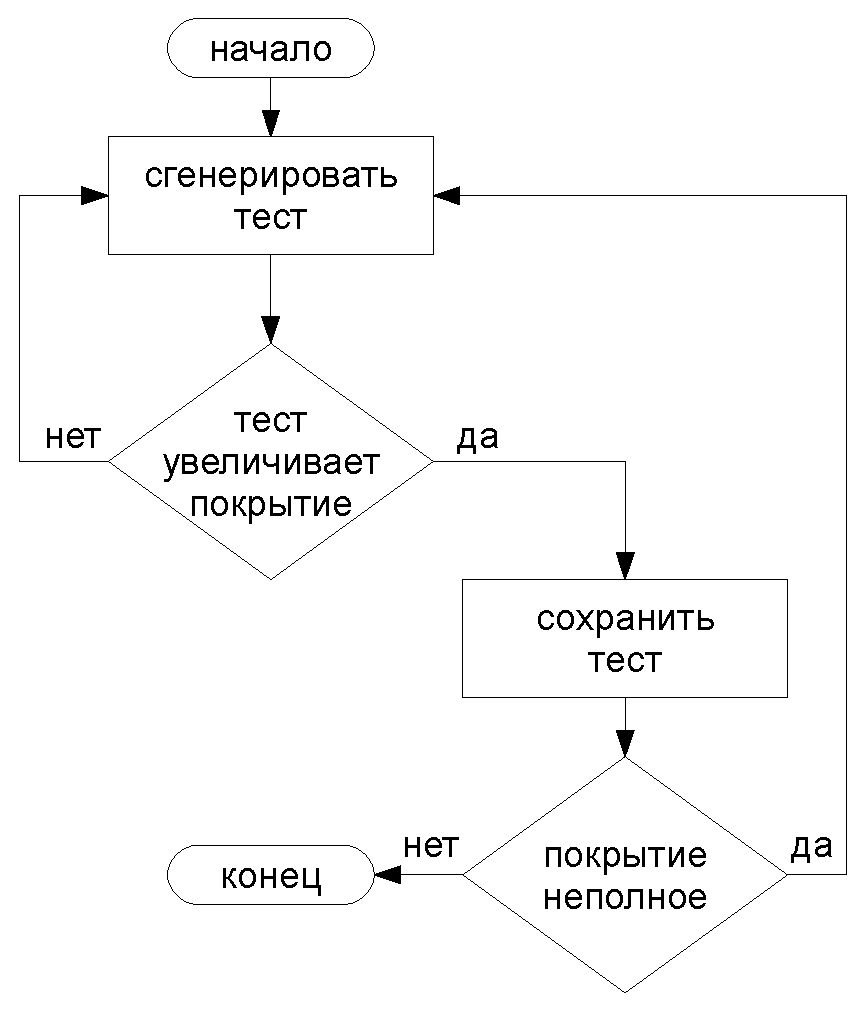
\includegraphics[width=0.45\textwidth]{1.review/methods1}\\
  \caption{Схема методов без выделения тестовых случаев}\label{fig:methods1}
\end{figure}

Схематично эти методы изображены на рисунке~\ref{fig:methods1}. В них чередуются этапы генерации тестов и их фильтрации по факту неувеличения покрытия. В каждом методе определяется своя процедура (массовой) генерации тестов. Процедура фильтрации основана на выбранном критерии покрытия (покрыта ли новая ошибка, покрыто ли новое требование, покрыта ли новая часть кода).

Наиболее очевидный метод генерации тестов --- (псевдо)случайная генерация. Этот метод подходит при любом критерии покрытия.

% авторы статьи, год статьи
% что тестировали ("тесты для такой-то подсистемы")
% из чего состоят тесты ("тесты состояли из .....")
% какое покрытие рассматривали ("тесты нацеливались на ...")
% каким способом генерировали тесты

В статье Д.Вуда, Г.Гибсона и Р.Каца из Университета в Беркли 1990 года описан метод генерации тестов~\cite{Berkeley89}, который использовался для верификации реализации протокола когерентности кэшей микропроцессоров SPUR, разрабатываемых также в Беркли. Тесты нацеливались на различные случаи взаимодействия микропроцессоров. Авторы отметили, что явное построение тестов для каждого отдельного случая взаимодействия микропроцессоров является тяжелой задачей. Вместо этого они предложили генерировать случайным образом программы для каждого микропроцессора в отдельности, аккуратно выбирая адреса ячеек памяти в инструкциях этих программ (чтобы в кэш-памяти разных микропроцессоров оказывались одни и те же <<адреса>> данных). Для этого сначала разработчики design'а пишут набор <<скриптов>>. Каждый скрипт состоит из двух программ: <<действия>> и <<проверки>>. В <<действии>> совершается некоторое тестовое воздействие, в <<проверке>> анализируется корректность изменения состояния микропроцессора в ответ на тестовое воздействие. Например, в <<действии>> происходит запись некоторого заданного значения по некоторому заданному адресу, а в <<проверке>> происходит считывание значения по этому адресу и проверка равенства этого значения записанному ранее. Затем генератор в случайном порядке выбирает <<действия>> и <<проверки>>, составляя тестовые программы.

%Еще две статьи по случайной генерации тестов для верификации блокировок в конвейере и арифметических алгоритмов (Maur88, Shal87 в статье Berkeley89)...............

П.Мишра и Н.Дутт в 2002 году предложили использовать model checking~\cite{ModelChecking} для генерации тестов~\cite{MishraDutt02}. Тесты нацелены на верификацию конвейеров. Покрытие измерялось по ситуациям в стадиях конвейера и в функциональных блоках. Генерацию тестов предлагалось делать следующим образом. Вручную на языке EXPRESSION~\cite{EXPRESSION} подготавливается описание архитектуры . Затем вручную (на языке SMV~\cite{SMV}) подготавливаются предикаты, выражающие ситуации в конвейере. После этого автоматически модель конвейера на EXPRESSION транслируется на SMV, для предикатов составляется их отрицание и модель вместе с ним подаются на вход инструмента SMV. Если инструмент доказывает выполнение поданного ему свойства в модели конвейера, значит в ней исходный предикат не выполнен (хотя должен бы) --- обнаружена ошибка. Если инструмент находит контрпример, то этот контрпример также автоматически транслируется в последовательность инструкций, т.е. тестовую программу. Полученная тестовая программа запускается на симуляторе (он автоматически получен по модели на EXPRESSION) с целью измерения покрытия. Если полученное покрытие недостаточно, надо вручную проанализировать его и построить дополнительные предикаты, и на них вновь провести всю эту схему. И так до тех пор, пока не будет получено нужное покрытие.

В 2003 году исследователями из Politecnico di Torino был предложен метод генерации тестовых программ с использованием генетических алгоритмов~\cite{microGP}. Тесты нацеливались на ошибки <<замыкания-в-0>> и <<замыкания-в-1>> вентилей схемы (stuck-at faults). В качестве хромосом рассматривались ациклические орграфы, вершинам которых приписаны инструкции (собственно, ген --- вершина этого орграфа). Мутация предполагает добавление, удаление или модификацию содержимого вершин. Кросс-овер понимается в виде замены подграфов. Функция отбора линейно зависит от количества обнаруживаемых хромосомой замыканий.

\subsection{Методы с выделением тестовых случаев}

\begin{figure}[h] \center
  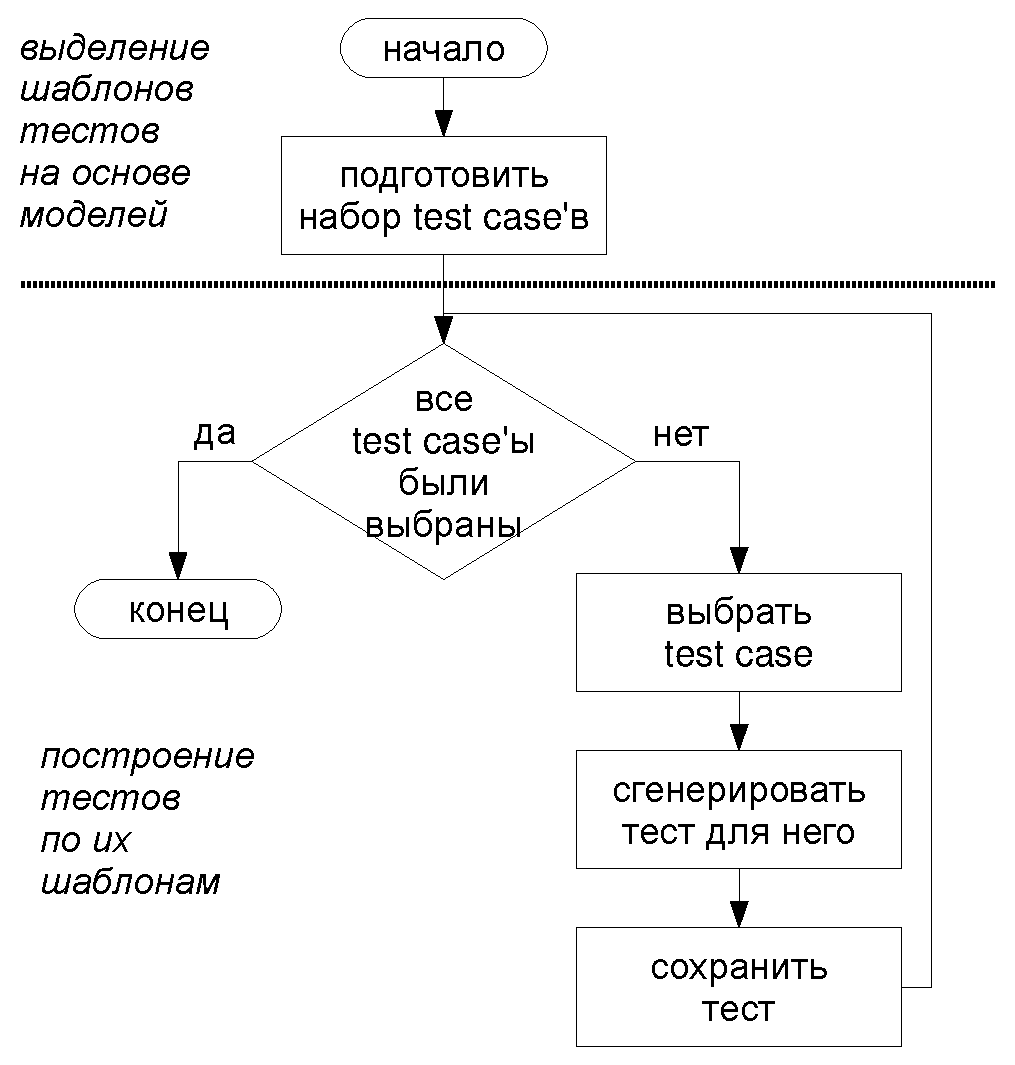
\includegraphics[width=0.45\textwidth]{1.review/methods2}\\
  \caption{Схема методов с выделением тестовых случаев}\label{fig:methods2}
\end{figure}

%Б) методы, которые выделяют элементы модели в виде шаблонов
Схематично эти методы изображены на рисунке~\ref{fig:methods2}. В каждом методе явно определяется критерий покрытия на основе некоторой модели (набор test case'в). Элементы покрытия (отдельные test case'ы) могут быть выделены как вручную, так и специальными алгоритмами на основе модели. Затем для каждого test case'а генерируется тест (тестовая программа) или набор тестов.

Любой метод без выделения тестовых случаев порождает метод с выделением тестовых случаев. Например, в таком методе для выбранного test case'а должны строиться тестовые программы до тех пор, пока не будет покрыт выбранный тестовый случай. Однако подобную реализацию построения тестов нельзя назвать эффективной (в противном случае, отдельное рассмотрение методов с выделением тестовых случаев было бы излишним).

%..... Подход Model-Based Testing~\cite{link!........}, поэтому составляется модель..........

В работах~\cite{UrFSM, mVpGen, MicroTESK} предлагаются методы для выполнения этапа для построения test case'в по моделям. Их обзору посвящен раздел~\ref{sec:templates_generation_methods}. В работах~\cite{MicroTESK, SEGUE1, SEGUE2, PA-RISC, TSE, Theo, mVpGen, GeneticTemplates, GenesysPro, GenesysPro2004Innovations, DeepTrans, RAVEN, MAATG} предлагаются методы для этапа построения тестов для test case'в. Их обзору посвящен раздел~\ref{sec:test_templates_generation_methods}. Обычно при таком разделении задачи построения тестов test case'ы представляются в виде \emph{шаблонов} тестовых программ (или, \emph{тестовые шаблоны}) --- параметризованных текстов тестовых программ. Выбором значений параметров по шаблону теста строятся тестовые программы. Оставшаяся часть этого раздела посвящена методам построения программ с выделением тестовых случаев, в которых этапы выделения test case'в и построения по ним программ сильно связаны.

% авторы статьи, год статьи
% что тестировали ("тесты для такой-то подсистемы")
% из чего состоят тесты ("тесты состояли из .....")
% какая модель микропроцессора используется (автоматы, графы, деревья инструкций)
% какое покрытие рассматривали ("тесты нацеливались на ...", что такое test case)
% каким способом генерировали тесты

П.Мишра и Н.Дутт в 2004 году предложили использовать model checking~\cite{ModelChecking} для генерации тестов~\cite{MishraDutt04}. Тесты нацелены на верификацию конвейера. Согласно подходу model-based testing, для конвейера составляется модель. Она представляет собой орграф. Его вершинами являются стадии конвейера, запоминающие устройства (например, кэш-память первого уровня), инструкции и их аргументы. Дуги соответствуют отношениям использования и порядка. На основе модели автоматически выделяются test case'ы. Для вершин и дуг графа в статье определен набор ситуаций --- эти ситуации и составляют test case. Генерация тестов происходит следующим образом. Вручную готовится модель конвейера на языке EXPRESSION~\cite{EXPRESSION}. По ней автоматически строится графовая модель. Из этой модели выделяются test case'ы, строится его отрицание, оно транслируется в формулу на языке SMV~\cite{SMV}. Эта формула и сгенерированная по модели конвейера на EXPRESSION модель на SMV подаются на вход инструменту SMV. Если доказано выполнение формулы, значит обнаружена ошибка. Если выполнение формулы не доказано, инструмент строит контрпример, подтверждающий исходный test case. Контрпример транслируется в тестовую программу и весь процесс продолжается для следующего test case'а. В дальнейших работах были предложены методы декомпозиции свойств и моделей и использование bounded model checking~\cite{Mishra09}.

Однако П.Мишра и Н.Дутт продолжили исследования, поскольку SMV (и другие современные инструменты model checking) не позволяют работать с более чем модельными примерами конвейеров. В работе 2005 года они опубликовали метод генерации тестов для верификации конвейеров уже без использования model checking~\cite{MishraDutt05}. Графовая модель конвейера осталась той же. Ее вершинами являются стадии, запоминающие устройства, инструкции и их аргументы. Дуги соответствуют отношениям использования и порядка. В статье были выделены 4 вида ошибок в конвейерах (чтение после записи в регистр дает другое значение, неверное вычисление операции, ошибки в активизации стадий конвейера, эффект <<параллельного>> исполнения инструкций) и требования на тестовые программы (test case'ы), на которых ошибки этих видов могут возникать. В статье описаны алгоритмы построения тестовых программ для каждого вида ошибок. Покрытие определяется на основе ситуаций в конвейере, которые определяют предложенные 4 вида ошибок. Суммируя вышесказанное, генерацию тестов предлагается делать следующим образом. Вручную готовится графовая модель конвейера и подается на вход алгоритма генерации программ для каждого вида ошибок. В этом алгоритме выделяются характерные последовательности инструкций и  дополняется до полных последовательностей инструкций (вставляются несущественные инструкции для заполнения промежутков, вычисляются нужные значения параметров и добавляются инструкции их инициализации).

В статье исследователей из Университета Карнеги-Меллон предложена методика построения тестовых программ для верификации подсистемы предсказания ветвлений~\cite{Branches99}. Методика была апробирована на микропроцессоре PowerPC 640. В этом микропроцессоре предсказание ветвлений выполняется с использованием двух кэшей. Для каждого из них авторы предлагают строить модели в виде конечных автоматов. Критерий покрытия определяется на основе этих автоматов (а именно, покрытие переходов). Авторы отмечают, что им удалось на тестах получить 100\% покрытие переходов автоматов. Предложенная ими методика построения тестов включает следующие шаги. Сначала подготавливаются модель подсистемы предсказаний ветвлений (набор конечных автоматов). Затем подготавливается набор программ для покрытия каждого отдельного перехода автомата. Далее надо реализовать и выполнить алгоритм, выбирающий некоторое множество путей в построенных конечных автоматах. И, наконец, выполнить (независимый от модели) алгоритм, который для выбранных путей и программ для отдельных переходов построит программы для каждого пути. Авторы отмечают, что эта методика применима в том числе для тестирования механизмов динамического переименования регистров и блокировок в конвейере.

\subsection{Методы выделения шаблонов на основе моделей}\label{sec:templates_generation_methods}

Часто шаблоны тестов строятся вручную. Это позволяет достаточно точно выразить требования к тестовым программам.

Ш.Ур и Й.Ядин в 1999 году предложили метод построения шаблонов тестов для верификации конвейеров на основе моделей~\cite{UrFSM}. В качестве моделей они предложили использовать конечные автоматы. Для определения автомата вводится набор переменных, состояние автомата представляется значениями этих переменных. Переход в автомате соответствует изменению значений переменных на очередном такте. Для компактного задания автомата в статье использован язык SMV~\cite{SMV}. Покрытие также строится на основе конечного автомата. А именно, элементом покрытия является путь, включающий изменение выделенного подмножества переменных (изменение полного набора переменных потребовало бы слишком большого количества тестов). Вручную надо построить модель конвейера (на SMV) и выбрать подмножество переменных. Выбор путей и построение тестовых программ будет выполнено автоматически. А именно, каждый выбранный путь будет преобразован в тестовый шаблон, а каждый построенный тестовый шаблон будет передан инструменту Genesys~\cite{GenesysPro} (о нём пойдет речь чуть позже), который построит тестовую программу.

%строим модель: переменные, они изменяются на каждом такте: есть init - начальные значения, есть next - значения переменных "на следующем такте". Получается, что на каждом такте изменяется значение каждой переменной. Иными словами получается конечный автомат, состояние которого есть вектор значений переменных. Может быть очень большой, но конечный автомат. Задается он, конечно же, не матрицей смежности, а функциями, которые строят новые значения переменных по старым. Далее выбираются некоторые переменные и покрытие строится только по тем переходам в автомате, где изменяются значения этих переменных?

К.Кохно и Н.Мацумото в 2001 году предложили свой метод построения тестовых шаблонов на основе модели конвейера~\cite{mVpGen}. Модель представляет собой конечный автомат. Состояниями автомата являются состояния конвейера (кортеж состояний стадий конвейера). Переходы между состояниями соответствуют изменению состояния конвейера на очередном такте. Переходы параметризованы инструкцией, поступающей на вход конвейера. Test case определяется как множество состояний автомата. Авторами выделены 3 вида test case'в (конфликты по данным, структурные конфликты, комбинации конфликтов по данным и структурных конфликтов) и алгоритмы определения множеств состояний автомата, представляющих каждый вид test case'в. Покрытие определяется на всех состояниях автомата, которые относятся к какому-либо виду test case'в. Элемент покрытия --- это одно состояние автомата. Пометки переходов пути из начального состояния в него дают последовательность (типов) инструкций тестового шаблона. Построение тестов осуществляется следующим образом. Вручную описывается <<поведенческая спецификация>> конвейера. На ее основе определяется структура автомата (явно автомат не строится, поскольку он имел бы слишком большие размеры). Затем определяется набор test case'в (состояний автомата). Для каждого test case'а строится тестовый шаблон, исходя из пути в автомате от начального состояния к состоянию test case'а. Тестовые шаблоны представляют собой последовательность типов инструкций с простейшими зависимостями между их аргументами (некоторые инструкции могут иметь одинаковые аргументы). Произвольным выбором инструкций соответствующих типов и аргументов тестовый шаблон преобразуется в тестовую программу.

А.Камкин в 2008 году предложил комбинаторный метод построения шаблонов тестов на основе модели микропроцессора~\cite{MicroTESK}. Модель представляет собой список (классов) инструкций, в котором для каждой инструкции указаны
\begin{itemize}
\item аргументы;
\item \emph{тестовые ситуации} --- ограничения на аргументы инструкции и состояние микропроцессора перед исполнением инструкции;
\item список зависимостей
    \begin{itemize}
    \item зависимости по аргументам (например, две инструкции используют один и тот же регистр);
    \item зависимости по адресам (например, одинаковые или разные виртуальные/физические адреса).
    \end{itemize}
\end{itemize}

Покрытие строится на основе модели микропроцессора. Тестовый шаблон (как элемент покрытия) представляет собой последовательность инструкций некоторой длины с выбранными для них зависимостями и тестовыми ситуациями. Построение тестов осуществляется по следующей схеме:
\begin{enumerate}
\item на основе модели комбинаторным образом строится множество шаблонов, т.е. перебираются все возможные последовательности (классов) инструкций с зависимостями и тестовыми ситуациями;
\item для каждого шаблона выбираются аргументы (конкретные регистры);
\item удовлетворяются зависимости по аргументам: зависимая инструкция получает значения аргументов инструкции, от которой она зависит;
\item удовлетворяются зависимости по адресам;
\item строятся подпрограммы подготовки инструкций (поместить нужные значения в регистры, в кэш-память и т.п.);
\item подпрограммы подготовки объединяются в единую инициализирующую программу.
\end{enumerate}

Методика предполагает ручное написание компонентов генератора тестов, осуществляющих отдельные этапы генерации, а именно, написание компонентов, удовлетворяющих зависимости, компонентов, строящих подпрограммы подготовки и др. В работе отмечается успешное применение методики для тестирования подсистемы управления памятью и конвейеров некоторых микропроцессоров архитектуры MIPS64~\cite{mips64II}.

\subsection{Методы построения теста по шаблону}\label{sec:test_templates_generation_methods}

Тестовые шаблоны --- это абстрактное представление тестовых программ. Обычно структура тестовых шаблонов повторяет структуру будущих тестовых программ. А именно, в тестовом шаблоне задана последовательность инструкций или типов инструкций (явно или неявно), свойства аргументов инструкций. В тестовом шаблоне могут быть заданы его динамические свойства (ограничения на состояния микропроцессора). В тестовой программе должна быть соблюдена последовательность инструкций и свойства аргументов, заданные в его тестовом шаблоне.

В литературе выделяются следующие методы построения тестовых программ по шаблонам:
\begin{enumerate}
	\item ручное написание генератора тестов~\cite{MicroTESK};
	\item псевдослучайное дополнение шаблона до теста~\cite{SEGUE1, SEGUE2, PA-RISC, TSE, Theo, mVpGen};
	\item использование генетических алгоритмов~\cite{GeneticTemplates};
	\item использование разрешения ограничений (constraints satisfaction~\cite{CLPusingECLiPSe})~\cite{GenesysPro, GenesysPro2004Innovations, DeepTrans, RAVEN, MAATG}.
\end{enumerate}

Довольно много работ следует методу псевдослучайного дополнения тестового шаблона до программы~\cite{SEGUE1, SEGUE2, PA-RISC, TSE, Theo, mVpGen}. В этом методе тестовый шаблон представляется в виде текста с вставками переменных. Задано множество значений для каждой переменной. Тестовая программа представляет собой тот же текст, но вместо переменных подставлено псевдослучайное значение из их множеств значений. Иными словами, построение теста заключается в наборе псевдослучайных текстуальных подстановках. Некоторые инструменты позволяют управлять псевдослучайным выбором с помощью указания вероятностей выбора некоторых значений. Авторы статей отмечают невысокую трудоемкостью и возможность тонкой настройки на получение нужных тестов.

В статье~\cite{GeneticTemplates} предложен метод дополнения тестового шаблона до программы с использованием генетического алгоритма. Вручную готовится набор <<макросов>> --- тестовых шаблонов. От тестовых программ их отличает лишь присутствие переменных на месте аргументов инструкций. Затем для каждого макроса с помощью генетического алгоритма ищутся значения аргументов, максимизирующих количество обнаруживаемых <<замыканий>> вентилей (<<замыканий-в-1>> и <<замыканий-в-0>>). В этом генетическом алгоритме хромосомой является кортеж значений переменных, функцией отбора является количество обнаруживаемых <<замыканий>> вентилей. Авторы советуют, чтобы в макросах как минимум встретились все инструкции.

%! еще ATPG ? Politectico di Milano \cite{toATPG}

Другой класс статей и инструментов следует методу, основанному на разрешении ограничений (constraints satisfaction~\cite{CLPusingECLiPSe})~\cite{GenesysPro, GenesysPro2004Innovations, DeepTrans, RAVEN, MAATG}. Как и прежде, тестовый шаблон содержит в себе информацию двух видов: параметрическую (шаблон --- это набор параметров, на значениях которых заданы отношения) и текстуальную (шаблон --- это будущий текст программы). В этом методе из тестового шаблона извлекается набор параметров, их множества значений и отношения на них. На этой основе строится система <<ограничений>> (constraints) на значения параметров. Ограничение --- есть ни что иное, как отношение, предикат. Разрешить ограничения --- значит подобрать значения параметров, на которых ограничение является истинным. Итак, разрешив выделенные для тестового шаблона ограничения, получаются значения параметров тестового шаблона. На заключительном этапе строится текст программы по вычисленным значениям параметров. Существование ряда эффективных процедур разрешения ограничений~\cite{CLPusingECLiPSe, SMT} определило и эффективное использование разрешения ограничений для построения тестовых программ.

Представленные методы обладают общими чертами: во всех них из тестового шаблона выделяется набор параметров, затем (различными способами) параметры получают некоторые значения и эти значения подставляются в тестовый шаблон. Методы, основанные на разрешении ограничений, позволяют задать в шаблонах более чётко допустимое множество значений параметров. Поэтому эти методы позволяют строить тестовые программы, нацеленные на более сложные ситуации поведения.

\section{Анализ существующих методов построения нацеленных тестов}

Проанализируем представленные в литературе методы генерации нацеленных тестов на предмет построения программ для тестирования подсистемы управления памяти. Грубо говоря, для тестирование корректности реализации кэширования и трансляции адресов. Для этого с помощью различных цепочек инструкций будут создаваться специальные ситуации в блоках подсистемы управления памяти.

Анализ будем проводить по следующим критериям:
\begin{itemize}
	\item применимость для ситуаций на подсистему управления памяти (как минимум, возможность составления тестовых программ с инструкциями обращения к памяти);
	\item масштабируемость по длине программы: работает ли метод для программ из 10-15 зависимых инструкций, что дает возможность тестировать подсистему управления памяти в ситуациях, нацеленных на различные буферы, размер которых (см.раздел~\ref{section:cache}) варьируется от 4-16 строк;
	\item масштабируемость по размеру кэш-памяти;
	\item возможность нацеливания на функциональность.
\end{itemize}

Согласно этим критериям методы без выделения тестовых шаблонов обладают следующими характеристиками:
\begin{itemize}
	\item метод, описанный в работе \cite{Berkeley89}, имеет узкую специализацию и не подходит для <<памяти>>;
	\item метод, описанный в работе \cite{MishraDutt02}, не масштабируем на реальные микропроцессоры, о чем говорят и сами авторы;
	\item метод, описанный в работе \cite{microGP}, предназначен для получения тестов, нацеленных на единичные замыкания схемы (stuck-at faults).
\end{itemize}

Методы с выделением тестовых шаблонов:
\begin{itemize}
		\item применение model checking~\cite{MishraDutt04} сталкивается с проблемами масштабирования, авторам приходится придумывать нетривиальные декомпозиции, чтобы повысить допустимый размер design'а;
		\item методы, описанные в работах~\cite{MishraDutt05, Branches99}, обладают узкой специализацией и не применимы для тестирования памяти;
		\item ручные методы написания генераторов тестов по шаблонам не масштабируемы по длине программы (количество зависимостей растет экспоненциально от длины шаблонов);
		\item методы псевдослучайного дополнения шаблонов не применимы для тестирования памяти, поскольку шаблоны включают в себя информацию о ситуациях в кэш-памяти, логика работы которой  не выражается в виде статических текстов с параметрами;
		\item применение методов, основанных на генетических алгоритмах, возможно, но надо чётко понимать, какая функция максимизируется, что неочевидно, ведь для данного шаблона надо построить всего одну тестовую программу --- произвольная тестовая программа либо соответствует шаблону, либо не соответствует, других вариантов нет; кроме того, при включении всей нужной информации в хромосому ее длина будет очень большой (в нее войдут начальное состояние микропроцессора и значения аргументов  инструкций --- их размер большой), что станет причиной плохой сходимости метода при <<глобальной>> функции отбора (включающей все гены хромосомы).
\end{itemize}

Методы, основанные на разрешении ограничений, были успешно применены для верификации реальных подсистем управления памяти (например, в PowerPC~\cite{GenesysPro}). Иными словами, они не только применимы, но и масштабируемы для реальных подсистем управления памяти.

%остаются constraints.

%метод построения шаблонов любой - все ли подходят для памяти?

Рассмотрим детальнее инструменты и методы, использующие разрешение ограничений, на предмет извлечения из них достаточных для воспроизведения описаний методов. Публикации по инструменту Genesys-Pro~\cite{GenesysPro, GenesysPro2004Innovations, GenesysSolver} оставляют достаточно много важных пробелов. Непонятно, каким образом происходит разрешение ограничений с массивами (а без таких ограничений не выразить ситуации в различных буферах данных). Этот инструмент не распространяется компанией IBM. По инструменту RAVEN публикаций в открытой научной печати с описанием, допустимым для возможности воспроизведения инструмента, нет вовсе~\cite{RAVEN} --- эти подробности являются коммерческой тайной. Инструмент MAATG является академической разработкой, по нему в открытой научной печати существует единственная работа~\cite{MAATG}, однако она не дает метод построения ограничений.

Таким образом, перспективными для построения нацеленных (на <<память>>) тестов являются  методы, включающие выделение отдельных тестовых шаблонов, а в качестве методов построения тестовой программы по тестовому шаблону --- разрешение ограничений. В этом классе методов нет открытых для науки методов.

%В) анализ: основываться будем на втором классе (почему он лучше? - для памяти подходит!)

%статья (1996)
%I’m Done Simulating;Now What? Verification Coverage Analysis and CorrectnessChecking of the DECchip 21164 Alpha microprocessor.
%описывает основные виды функциональной верификации:
%* assertions в RTL
%* самопроверяющиеся тесты
%* сравнение с эталоном
%
%В ней указываются методы псевдослучайно генерации тестов:
%
%W. Anderson, "Logical Verification of the NVAX CPU Chip
%Design," Digital Technical Journal, vol. 4, no. 3 (Summer 1992):
%38-46.
%-------------
%SEGUE - инженеры составляют набор шаблонов программ, которые вызывают разные события. В этих шаблонах вместо инструкций могут указываться лишь типы инструкций, вместо аргументов некий "произвольный аргумент".
%Шаблон верхнего уровня указывает, с какими вероятностями должны встречаться шаблоны нижнего уровня (которые писали для возникновения событий).
%Демоны моделируют псевдослучайное поведение среды, в которой работает микропроцессор.
%-------------
%
%4. A. Ahi, G. Burroughs, A. Gore, S. LaMar, C-Y. Lin, and A.
%Wiemann, "Design Verification of the HP 9000 Series 700 PARISC
%Workstations," Hewlett-Packard Journal (August 1992):
%34-42.
%-----
%похожее, но в HP
%-----
%
%5. D. Wood, G. Gibson, and R. Katz, "Verifying a Multiprocessor Cache Controller Using Random Test Generation," IEEE Design and Test of Computers (August 1990): 13-25.
%------------
%"модель" -- all multiprocessor interaction cases
%архитектура SPUR
%-----------
%
%тесты из одной инструкции (1982!):
%D. Bhandarkar, "Architecture Management for Ensuring Software Compatibility in the VAX Family of Computers," IEEE Computer (February 1982): 87-93.
%
%random test generation for check pipeline interlocks and arithmetic algorithms
%[TBD!] Maurer, Design Verification of the WE32106 Math Accelerator Unit
%[TBD!] Shalem Carmon, Testing the Design of the NS32532 Microprocessor
%
%S. Taylor et al. “Functional verification of a multiple-issue, out-of-order, superscalar Alpha processor - the DEC Alpha 21264 microprocessor.” In Proc. DAC, 1998, pp. 638–643.
%----
%SEGUE - но на следующем микропропессоре
%------
%
%2009:Yingpan Wu, Lixin Yu, Wei Zhuang, Jianyong Wang, "A Coverage-Driven Constraint Random-Based Functional Verification Method of Pipeline Unit," icis, pp.1049-1054, 2009 Eigth IEEE/ACIS International Conference on Computer and Information Science (icis 2009), 2009
%
%
%Mishra, Dutt:
%Generation of effective test programs for the self-test of a processor has been studied by several researchers ([2] [18] [20] [21]).
%
%Ur and Yadin [23] presented a method for generation of assembler test programs that systematically probe the micro-architecture of a PowerPC processor.
%
%Iwashita et al. [3] use a FSM based processor modeling to automatically generate test programs.
%
%================
%Alpha 21164 (21264): I’m Done Simulating;Now What? Verification Coverage Analysis and CorrectnessChecking of the DECchip 21164 Alpha microprocessor.
%NVAX: W. Anderson, "Logical Verification of the NVAX CPU Chip Design," Digital Technical Journal, vol. 4, no. 3 (Summer 1992):38-46.
%HP 9000 Series 700 PARISC:  4. A. Ahi, G. Burroughs, A. Gore, S. LaMar, C-Y. Lin, and A. Wiemann, "Design Verification of the HP 9000 Series 700 PARISC Workstations," Hewlett-Packard Journal (August 1992): 34-42.
%PowerPC, VLIW: что-то Genesys 2005
%Intel использует тесты: http://www.cs.rice.edu/~vardi/comp607/bentley.pdf


\section{Уточненная постановка задачи}

В результате анализа существующих работ в предыдущем разделе был сделан вывод о перспективности определенного класса методов построения тестовых программ. Однако далеко эти методы не описаны настолько, чтобы была возможна отдельная от их авторов реализация. Исходя из этого вывода, в данной работе следует уточнить задачи. А именно, для разработки метода построения тестовых программ нужны:
\begin{enumerate}
	\item методы описания моделей подсистемы управления памяти;
	\item определение шаблонов и метод построения шаблонов на основе моделей;
	\item метод построения тестовой программы по шаблону.
\end{enumerate}

Второй пункт подробно описан в работе~\cite{MicroTESK} и далее рассматриваться не будет. Остальные два пункта дают уточненную постановку задачи в диссертации:
\begin{enumerate}
	\item предложить метод описания моделей подсистемы управления памяти (ее решению посвящен раздел~\ref{sec:state_model_section});
	\item предложить метод построения тестовой программы по шаблону (ее решению посвящена практически целиком следующая глава за исключением раздела~\ref{sec:state_model_section}).
\end{enumerate}

